%
% euler.tex
%
% (c) 2024 Prof Dr Andreas Müller
%
\begin{figure}
\centering
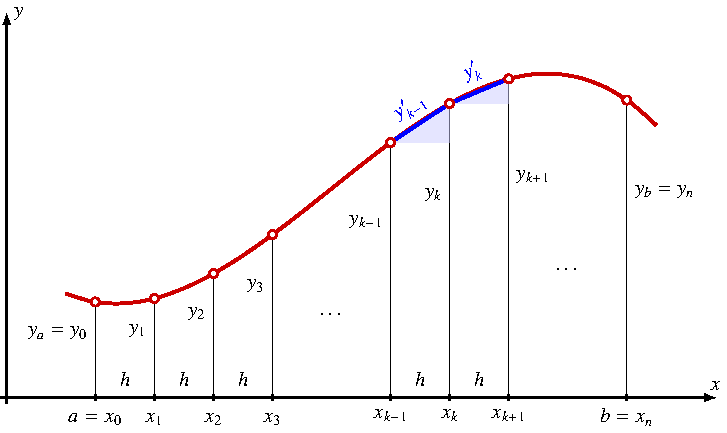
\includegraphics{chapters/070-direkt/images/euler.pdf}
\caption{Diskretisation der Lösungsfunktion für das Funktional
$I(y)$ von \eqref{buch:direkt:euler:eqn:aufgabe}, mit der Leonhard
Euler die Euler-Lagrange-Differentialgleichung hergeleitet hat.
\label{buch:direkt:euler:fig:euler}}
\end{figure}
